\chapter{Introduction}
\label{chap:intro}

Ce mémoire a pour but de retracer les missions réalisées durant mon stage de Master 2 Informatique pour l'Image et le Son à l'Université de Bordeaux 1, effectué entre Avril et Septembre 2018 (six mois), dans la société \texttt{RealityTech}\footnote{\href{http://rea.lity.tech/}{http://rea.lity.tech/}}. Ce rapport ne couvrira cependant que les cinq premiers mois du stage car la date de rendu de ce dernier précède d'un mois la date de fin du stage.\\

Le stage a donc été effectué chez \texttt{RealityTech} une jeune start-up de réalité augmentée spatiale créée fin 2016, ne comptant actuellement aucun employé. Issue de l'\texttt{Inria} de Bordeaux, l'institut national de la recherche en informatique et en automatique, cette dernière est la continuité d'un projet de recherche mené par M. Laviole, ex ingénieur de recherche à l'\texttt{Inria}. Ce projet, \texttt{PapARt}\footnote{\href{https://project.inria.fr/papart/fr/}{https://project.inria.fr/papart/fr/}} \emph{Paper Augmented Reality Toolkit}, est un kit de développement ou \emph{Software Development Kit (SDK)} \texttt{Processing} permettant de créer des expériences de réalité augmentée sous forme d'applications de projection interactive sur des feuilles de papier. Pour réaliser ce type d'application, du matériel spécifique est nécessaire tel que des caméras couleur et des caméras de profondeur qui sont utilisées pour capter le monde réel, un projecteur utilisé pour pouvoir visualiser le contenu numérique dans l'espace ainsi qu'un ordinateur pour effectuer tous les calculs nécessaires au bon fonctionnement des applications.\\

C'est, dans un premier temps, du côté matériel que \texttt{RealityTech} intervient. En effet, celle-ci propose des systèmes pré-calibrés et prêts à l'emploi résolvant ainsi tous les problèmes de calibration et d'installation de l'environnement nécessaire à l'utilisation de \texttt{PapARt}. En parallèle de la partie matérielle, la société développe et améliore activement le kit et créé également diverses applications de démonstration, afin de présenter et d'étendre les possibilités de la technologie. Le but est de pouvoir ouvrir la technologie à d'autres domaines d'activité que celui de la recherche, pour mettre les outils collaboratifs et les systèmes interactifs au service de l'éducation, du vidéo ludique, de la vulgarisation etc.

\section{Contexte et cadre}
\label{sec:contexte}
Actuellement, \texttt{RealityTech} se développe dans un incubateur de start-up appelé \texttt{La Banquiz}\footnote{\href{http://labanquiz.com}{http://labanquiz.com}}, situé 4 rue Eugène et Marc Dulout, à Pessac Centre. L'objectif de \texttt{La Banquiz} est de promouvoir des start-up Open Source\footnote{\href{https://fr.wikipedia.org/wiki/Open\_source}{Open Source - Wikipédia}} et innovantes en apportant à leurs dirigeants des formations, du coaching individuel et collectif, de l'aide pour la recherche de financement et tout ce qui gravite autour de l'accompagnement des jeunes entreprises.\\

À ce jour, \texttt{RealityTech} ne travaille qu'avec des laboratoires de recherche tel que l'\texttt{Inria} et cherche à étendre son secteur d'activité. Les systèmes et services proposés par la société fournissent les résultats espérés et la dynamique de celle-ci s'oriente donc vers une industrialisation du produit. Ainsi, l'entreprise souhaite passer de prototypes FabLab créés à l'unité basés sur des technologies de recherche, à des prototypes industriels basés sur des technologies populaires dans le monde de l'industrie. \texttt{RealityTech} se lance donc dans la création d'une plateforme haute performance appelée \texttt{Nectar} et dans le développement d'un nouvel \emph{SDK} \texttt{Unity}\footnote{\href{https://unity3d.com/fr}{https://unity3d.com/fr}} utilisant cette plateforme. Le \emph{SDK} \texttt{Processing} actuel est très accessible et permet de prototyper bon nombre d'applications rapidement, mais il ne permet cependant pas de répondre aux besoins de l'industrie, plus spécialement quand il s'agit de développer des applications client ayant besoin d'un moteur 3D ou d'un moteur physique performant.\\

Pour débuter ce stage, j'ai eu l'occasion de partir à Laval durant une semaine pour participer au \texttt{Laval Virtual}\footnote{\href{https://www.laval-virtual.org/}{https://www.laval-virtual.org/}}, le plus grand salon international sur la réalité augmentée et virtuelle, en tant qu'exposant. Grâce à ce salon, j'ai pu développer une bonne connaissance du produit et ai pu observer de nombreuses technologies à l'état de l'art dans ces domaines. Ce salon m'a également permis de bien comprendre les besoins auxquels pouvait répondre une technologie comme celle de \texttt{RealityTech} et par la même occasion les enjeux et les apports de celle-ci. Cela a aussi été une très bonne expérience sur le plan relationnel car elle m'a aidé à créer rapidement une relation avec M. Laviole, mon tuteur de stage.

Le reste de mon stage s'est déroulé à \texttt{La Banquiz} où j'ai été au contact de toutes les entreprises officiant en son sein. J'ai notamment pu rencontrer d'autres stagiaires tels que Rémi Kressmann, développeur, et Gabin Andrieux, commercial chez \texttt{LockEmail}\footnote{\href{http://www.lockemail.fr/}{http://www.lockemail.fr/}}, une entreprise de cyber-sécurité, mais aussi des dirigeants comme Jean François Schaff, docteur en physique quantique ayant créé  \texttt{Postelo}\footnote{\href{https://www.postelo.fr/}{https://www.postelo.fr/}} une plateforme de télé expertise pour les professionnels de santé, avec qui j'ai énormément échangé aussi bien sur des concepts de programmation, que sur la culture de l'informatique en général.

\section{Objectifs}

Au cours de ce stage, j'ai eu l'occasion de remplir bon nombre de tâches diverses et variées, guidées par les besoins de la société. Les tâches principales sont décrites dans le diagramme de Gantt effectif (Figure~\ref{fig:gantshort}) des cinq premiers mois de ce stage. Une version plus détaillée du diagramme et des tâches réalisées est disponible Annexe~\hyperref[annexe:gantt]{4}.

\begin{figure}[H]
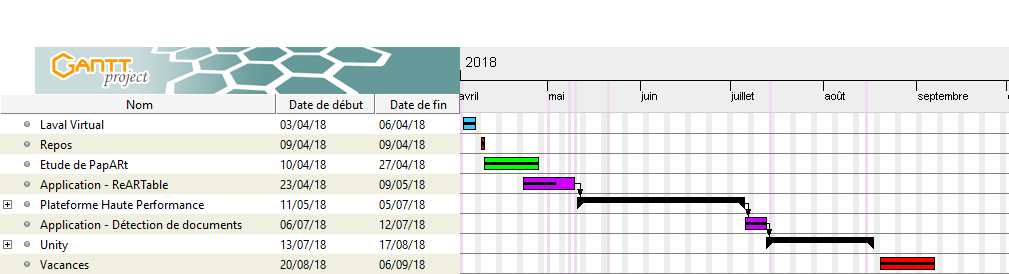
\includegraphics[width=\linewidth]{images/GanttMemoire}
\caption{Diagramme de Gantt effectif des tâches réalisées}
\label{fig:gantshort}
\end{figure}

\paragraph{Applications de démonstration} Le stage a débuté par le développement d'applications de démonstration en utilisant le système de l'entreprise (Chapitre~\ref{chap:app}). Le but était de comprendre l'essence, le fonctionnement global du système et ce qu'il était possible/impossible de réaliser avec celui-ci. Ainsi, en réalisant les tâches qui m'ont été confiées, j'ai pu acquérir à la fois une vision globale de l'architecture logicielle, du fonctionnement interne du kit de développement et de l'architecture matérielle nécessaire à son utilisation. Cela m'a également aidé à développer une certaine autonomie pour la suite du stage.

\paragraph{Plateforme haute performance} J'ai été amené à réaliser une preuve de concept visant à présenter une version haute performance du produit de l'entreprise (Chapitre~\ref{chap:protoHP}). Cette preuve de concept devait proposer des méthodes et des pistes d'amélioration de la solution actuelle aussi bien sur le plan logiciel, avec par exemple l'optimisation d'algorithmes existants (section~\ref{sec:hpsoft}), que sur le plan matériel, avec la réalisation de tests de performance des différents dispositifs d'acquisitions (section~\ref{sec:hardwareup}) que sont la caméra, le projecteur ainsi que sur l'architecture globale de la solution, où il a fallu développer une toute nouvelle architecture en microservices incluant un tout nouvel environnement de travail, ainsi qu'un gestionnaire de processus et un serveur web (section~\ref{sec:nectararchi}).

\paragraph{Kit de développement} Comme précédemment expliqué dans le contexte du stage, les besoins auxquels répond le kit de développement \texttt{Processing} actuellement en place ne sont plus suffisants lorsqu'il est question d'applications devant faire le rendu de grosses scènes 3D ou des simulations physiques par exemple. Le développement d'une version \texttt{Unity} du kit, permettant de créer des applications de projection interactive, s'est donc avéré nécessaire pour la suite du développement de \texttt{RealityTech} (Chapitre~\ref{chap:unity}). Pour que le développement de ce module soit efficace, l'objectif était d'intégrer et d'utiliser les microservices de la plateforme haute performance \texttt{Nectar} pour gérer tout ce qui concerne le monde physique (caméras, projecteurs, suivi d'objet, événements de toucher, etc.) et d'utiliser \texttt{Unity} dans son rôle de moteur 3D et de moteur physique pour gérer le rendu, la physique des objets, la lumière ainsi créer des expériences de projection encore plus évoluées. Le module devait également permettre d'ouvrir la technologie de \texttt{RealityTech} à un plus grand nombre d'utilisateur du fait de la notoriété d'\texttt{Unity} dans son domaine.\\

\begin{center}
Au vu de ces objectifs, il en découle que la problématique générale du stage est le développement d'applications et de technologies de réalité augmentée spatiale.
\end{center}

La présentation de ce mémoire sera divisée en plusieurs parties. Dans un premier temps, nous présenterons le domaine d'activité dans lequel s'insère ce stage en définissant les concepts clés nécessaires à la bonne compréhension de notre sujet. Ceci débouchera sur une revue des technologies existantes en la matière. Par la suite, les objectifs susmentionnés seront développés dans des parties spécifiques. Ainsi, le développement d'application, la création du prototype haute performance et du module \texttt{Unity} feront l'objet d'une présentation approfondie, retraçant les étapes de leur création ainsi que les difficultés méthodologiques auxquelles nous avons été confrontés. Enfin, nous conclurons en exposant les bénéfices aussi bien personnels que professionnels que ce stage m'a apporté.